%Dokumentinnstillinger:---------------------------------
%Ved å google flitting kan du finne ut hva de forskjellige tingene her betyr, og hvordan du kan gjøre eventuelle endringer.
\documentclass[a4paper,11pt,norsk]{article}
\usepackage[utf8]{inputenc}
\usepackage{a4wide}
\usepackage{lmodern}
\usepackage[T1]{fontenc}
\usepackage{babel}
\setlength{\parindent}{0pt} 
\setlength{\parskip}{2ex}
\usepackage{fixltx2e}
\usepackage{amsmath}
\usepackage[pdftex, pdfborderstyle={/S/U/W 0}]{hyperref}
\usepackage{graphicx}
\usepackage[font=small,labelfont=bf]{caption}
\usepackage{tabularx}
\usepackage{multirow}
\usepackage{float}
\usepackage[RPvoltages]{circuitikz}




\begin{document}

%Headingdel:---------------------------------------------
\begin{minipage}[c]{0.15\textwidth}

\includegraphics[width=2.0cm]{D1/Images/elsys_pos_staaende_ntnu.png}  
\end{minipage}
\begin{minipage}[c]{0.85\textwidth}

\renewcommand{\arraystretch}{1.7}
\large 
\begin{tabularx}{\textwidth}{|X|X|}
\hline
\multicolumn{2}{|l|}{} \\
\multicolumn{2}{|l|}{\huge \textbf{Designnotat}} \\
\multicolumn{2}{|l|}{}  \\
\hline
\multicolumn{2}{|l|}{Tittel: 
%Skriv inn tittel her:------------------------------------------
Støyfjerningsfilter
} \\
\hline
\multicolumn{2}{|l|}{Forfatter: 
%Skriv inn forfattere her:--------------------------------------
Freider Engstrøm Fløan
} \\
\hline
%Skriv inn versjon og dato her her:-----------------------------
Versjon: 2.0 & Dato: 01.05.22
\\
\hline 
\end{tabularx}
\end{minipage}
\normalsize

%Automatisk generert innholdsfortegnelse:------------------

\setlength{\parskip}{0ex}
\renewcommand{\baselinestretch}{0.1}\normalsize
\tableofcontents
\renewcommand{\baselinestretch}{1.00}\normalsize
\setlength{\parskip}{2ex}
\rule{\textwidth}{1pt}
\label{sec:innledning}

\newpage



%Selve rapporten:------------------------------------------
\section{Problembeskrivelse}
\label{sec:problembeskrivelse}

Vi vil ta for oss design av et system, vist i figur \ref{fig:1}, som skal fjerne uønsket støy fra et lydsignal. Systemet tar inn et signal $x(t)$, fjerner uønskede frekvenser  og gir ut et signal $\hat{s}(t)$, der de resterende frekvensene i lydsignalet forblir mest mulig uendret. 

\begin{figure}[H]
  \centering
  \includegraphics[scale=0.8]{D1/Images/InkedFig 1 støyfjerning_LI.jpg}
  \caption{System for filtrering av støy.}
  \label{fig:1}
\end{figure}

\section{Prinsipiell løsning}
\label{sec:prinsipielllosning}

Ved å utnytte egenskapene til linære kretskomponenter kan frekvenser både blokkeres og forbli uendret ut ifra hvordan de er koblet sammen. Ved hjelp av et båndstopp-filter kan frekvenser innenfor en båndbredde mellom $f_{L}$ og $f_H$ dempes til ønskelig nivå.  

\begin{figure}[H]
  \centering
  \includegraphics[scale=0.3]{D1/Images/InkedbåndstopEks_LI.jpg}
  \caption{Eksempel på amplitude og faserespons til et båndstopp-filter i et bodediagram.}
  \label{fig:2}
\end{figure}

Figur \ref{fig:2} viser eksempelvis et systems amplitude- og faserespons med bestemt $f_C$, der $f_L$ og $f_H$ er definert som frekvensene systemet demper amplituden med $-3 dB$.

Det finnes flere måter å designe kretser med båndstopp-filter som funksjon. Et eksempel på en slik krets, som vil bli brukt i realiseringen er vist i figur \ref{fig:3} under. Når 

\begin{figure}[H]
  \centering
  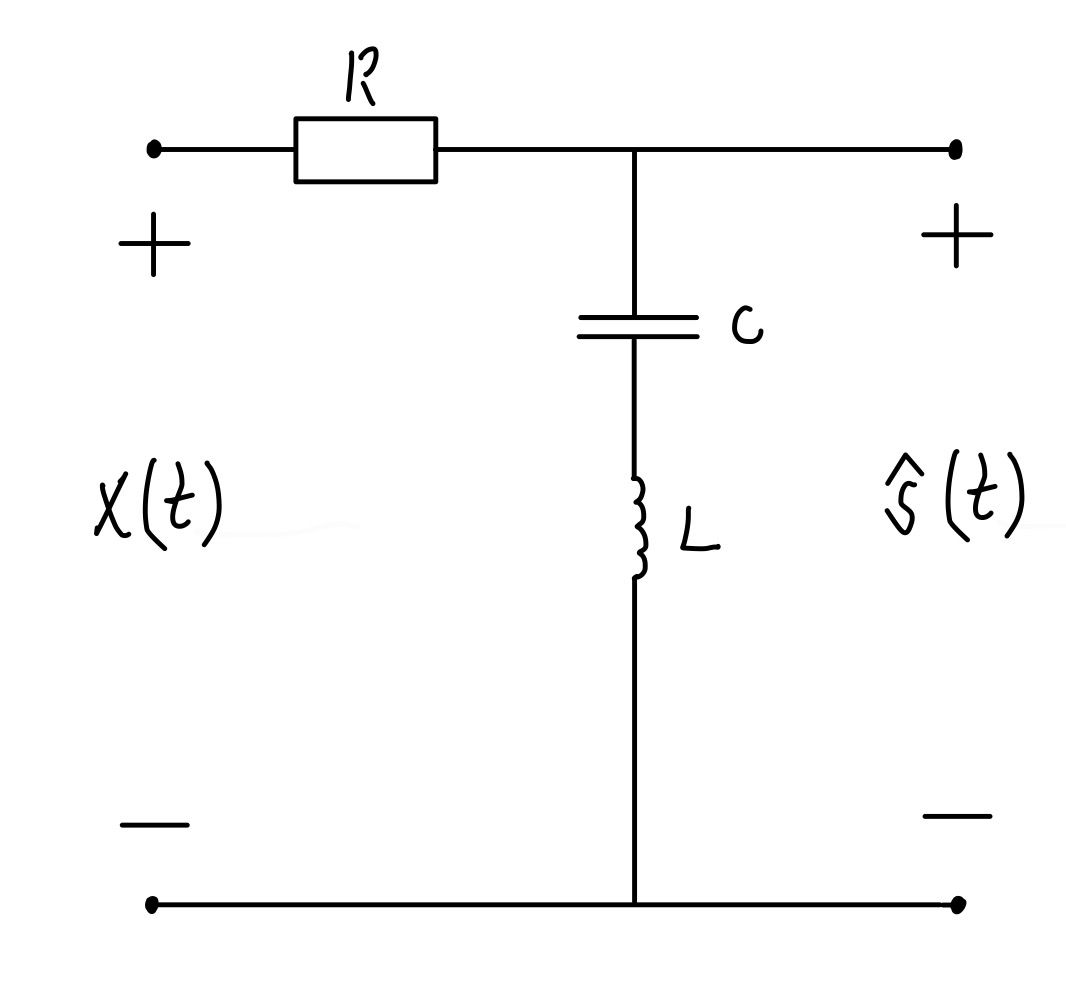
\includegraphics[scale=0.2]{D1/Images/IMG_E0537.JPG}
  \caption{Båndstopp-filter med en resistor, kondensator og spole.}
  \label{fig:3}
\end{figure}

Ved å ta utgangspunkt i kretsen i figur \ref{fig:3} og se på impedansen til kondensatoren og spolen, og derifra finne frekvensen der begge komponentene resonerer. Dette skjer når henholdsvis spolen og kondensatorens faserespons er 180 grader mot hverandre som vist i figur \ref{fig:2} ved $f_C$.

Impedansene til systemet i figur \ref{fig:3} er gitt ved
\begin{equation}
Z_R = R
\label{eq:1}
\end{equation}
\begin{equation}
Z_C = \frac{1}{j\omega C} 
\label{eq:2}
\end{equation}
\begin{equation}
Z_L = j\omega L
\label{eq:3}
\end{equation}
der vinkelfrekvensen $\omega$ $=$ $2\pi f$ og det komplekse tallet $j$ $=$ $\sqrt{-1}$. 

$\hat{s}(t)$ måles over kondensatoren og spolen i serie som kan regnes ut ved hjelp av amplituden til frekvensresponsen $|H(\omega)|$ og spenningsdeling:
\begin{equation}
    |H(\omega)|=\frac{|Z_C + Z_L|}{|Z_C+Z_L+Z_R|}x(t)
\end{equation}

\begin{equation}
    \hat{s}(t) = |H(\omega)|x(t)
\end{equation}

\begin{equation}
    \hat{s}(t) = \frac{|Z_C + Z_L|}{|Z_C+Z_L+Z_R|}x(t)
    \label{eq:4}
\end{equation}

Setter deretter inn impedansene (\ref{eq:1}), (\ref{eq:2}) og (\ref{eq:3}) i likning (\ref{eq:4})

\begin{equation}
    \hat{s}(t) = \frac{|\frac{1}{j\omega C} + j\omega L|}{|\frac{1}{j\omega C}+j\omega L+R|}x(t)
\end{equation}

som kan forenkles til

\begin{equation}
    \hat{s}(t) = \frac{x(t)}{\sqrt{1+\frac{R^2}{(\omega L - \frac{1}{\omega C})^2}}}
    \label{eq:5}
\end{equation}

Likning (\ref{eq:5}) gir at systemet avhenger av både $R$, $C$ og $L$. Hvis verdien til $R$ \xrightarrow $0$ vil $x(t)$ \xrightarrow $\hat{s}(t)$. Størrelsen på $R$ vil bestemme hvor stor demping som skjer ved $f_C$, samtidig som det endrer båndbredden. Dermed er størrelsen til $R$ avhengig av hvor stor demping og båndbredde systemet har behov for. En løsning på dette kan være å bruke en variabel motstand slik at man kan endre på båndbredden og dempingen, samtidig som man observerer endringer på signalet til man får et tilfredstillende resultat. 

Systemet i figur \ref{fig:3} gir en relativt bred båndbredde, derfor kan det være lurt å sette flere slike filter i serie for å øke dempingen ved $f_C$. Ved seriekobling av filter kan det være hensiktsmessig å legge inn en buffer, ved hjelp av en operasjons forsterker, mellom filtrene da tilkoblet last på systemet kan trekke mye strøm som kan føre til at signalstyrken minker (\textit{Enkle prinsipper for støyfjerning} av Lars Lundheim \cite{notat}). 

Ønsket amplituderespons ved $f_C$ er så lav som mulig, noe som oppnås når $L$ og $R$ resonerer og fungerer som en kortslutning slik at $\hat{s}(t)$ \xrightarrow $0$ ved $f_C$.
Ved å se på når telleren til $(\omega L - \frac{1}{\omega C})^2$ i (\ref{eq:5}) og telleren i (\ref{eq:4}) \xrightarrow $0$ er det mulig å regne ut $f_C$:
\begin{equation}
    \frac{1}{\omega C} + \omega L = 0
\end{equation}
\begin{equation}
    \frac{1}{2\pi f_C C} + 2 \pi f_C L = 0
\end{equation}

\begin{equation}
        f_C = \frac{1}{2\pi\sqrt{LC}}
        \label{eq:f_c}
\end{equation}

En ferdig krets vil da se ut som figur \ref{fig:4}, med ønskelig antall filtre i serie ut i fra hvor mye demping og hvor bred båndbredde som er nødvendig.

\begin{figure}[H]
  \centering
  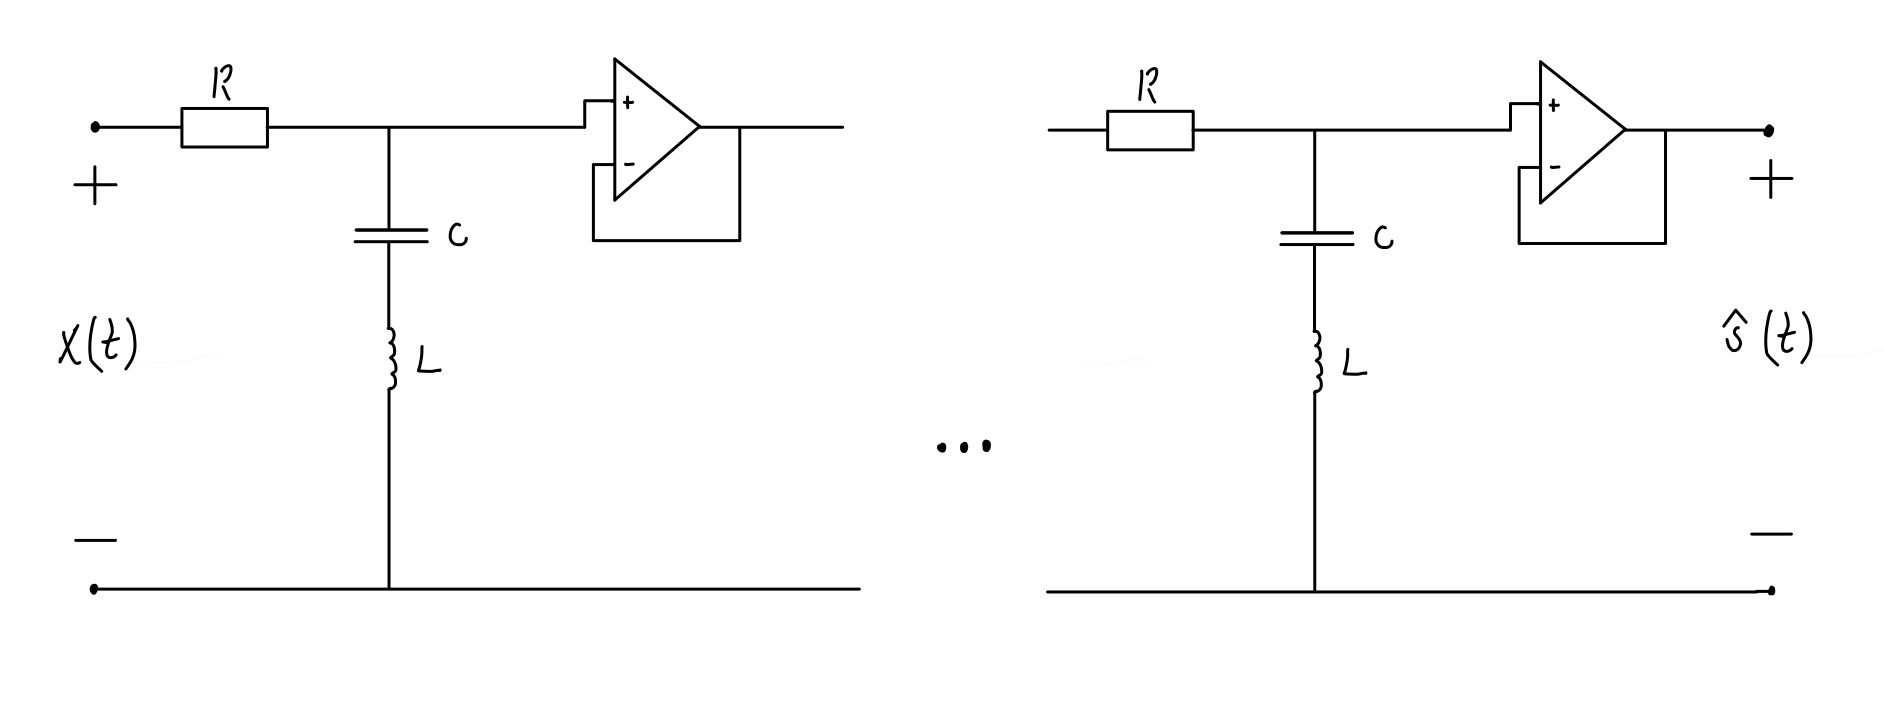
\includegraphics[scale=0.2]{D1/Images/IMG_E0539.JPG}
  \caption{Flere båndstopp-filter i serie med buffere imellom.}
  \label{fig:4}
\end{figure}

\section{Realisering og test}
\label{sec:realisering}
\subsection{Realisering}
Signalet som skal testes gjennom realisert system er et ti sekunders lydklipp av en sang med en konstant pipetone som skal fjernes. 
Ved hjelp av en spektrumanalysator er det mulig å identifisere frekvensen til den konstante pipetonen som vist i figur \ref{fig:5}.

\begin{figure}[H]
  \centering
  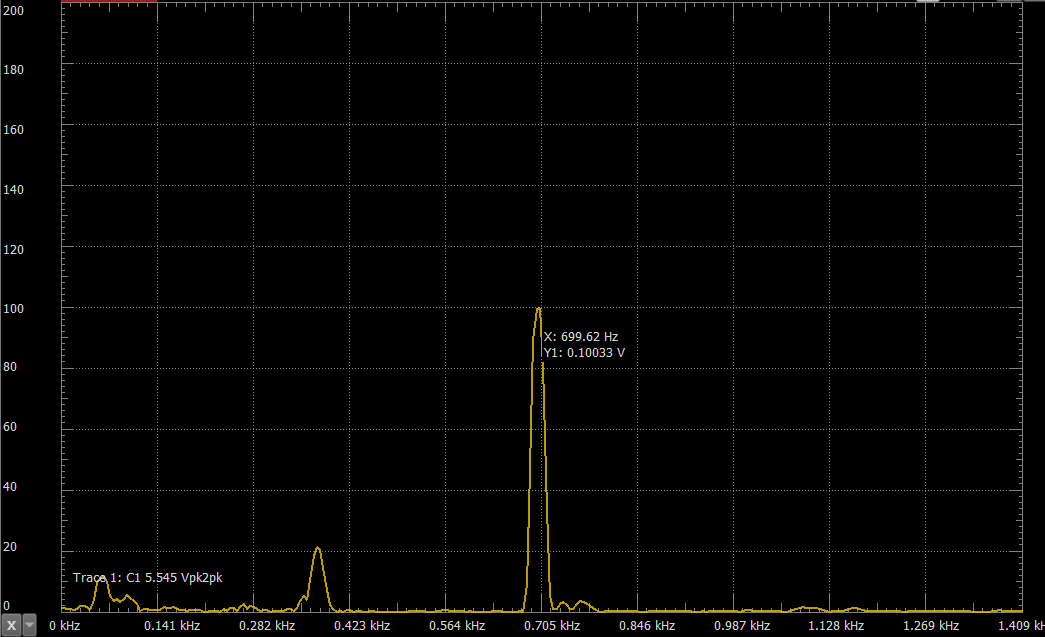
\includegraphics[scale=0.7]{D1/Images/Spectrum Analyzer 700Hz.png}
  \caption{Spektrumanalysator i programmet \emph{Waveforms}.}
  \label{fig:5}
\end{figure}

Spektrumanalysatoren i figur \ref{fig:5} identifiserte den uønskede pipetonen $f_C$ til å være $700Hz$. Med $f_C$ tilgjengelig kan likningen (\ref{eq:f_c}) brukes for å regne ut kondensator og spole verdi. 
Med en spole på $206mH$ allerede tilgjengelig kan kondensatorverdiene regnes ut
\begin{equation}
    f_C = \frac{1}{\sqrt{2\pi LC}}
\end{equation}
\begin{equation}
    \sqrt{LC}= \frac{1}{2\pi f_C}
\end{equation}
\begin{equation}
    C = \frac{1}{L(2\pi f_C)^2}
\end{equation}
Setter inn verdier for $L$ og $f_C$.
\begin{equation}
    C = \frac{1}{206mH(2\pi 700Hz)^2} \approx 251nF
\end{equation}

Realisering av systemet er vist i figur \ref{fig:oppkobling} med skjematisk oppkobling vist i figur \ref{fig:schematic} og komponentverdier i tabell \ref{tab:komp}.

\begin{figure}[H]
  \centering
  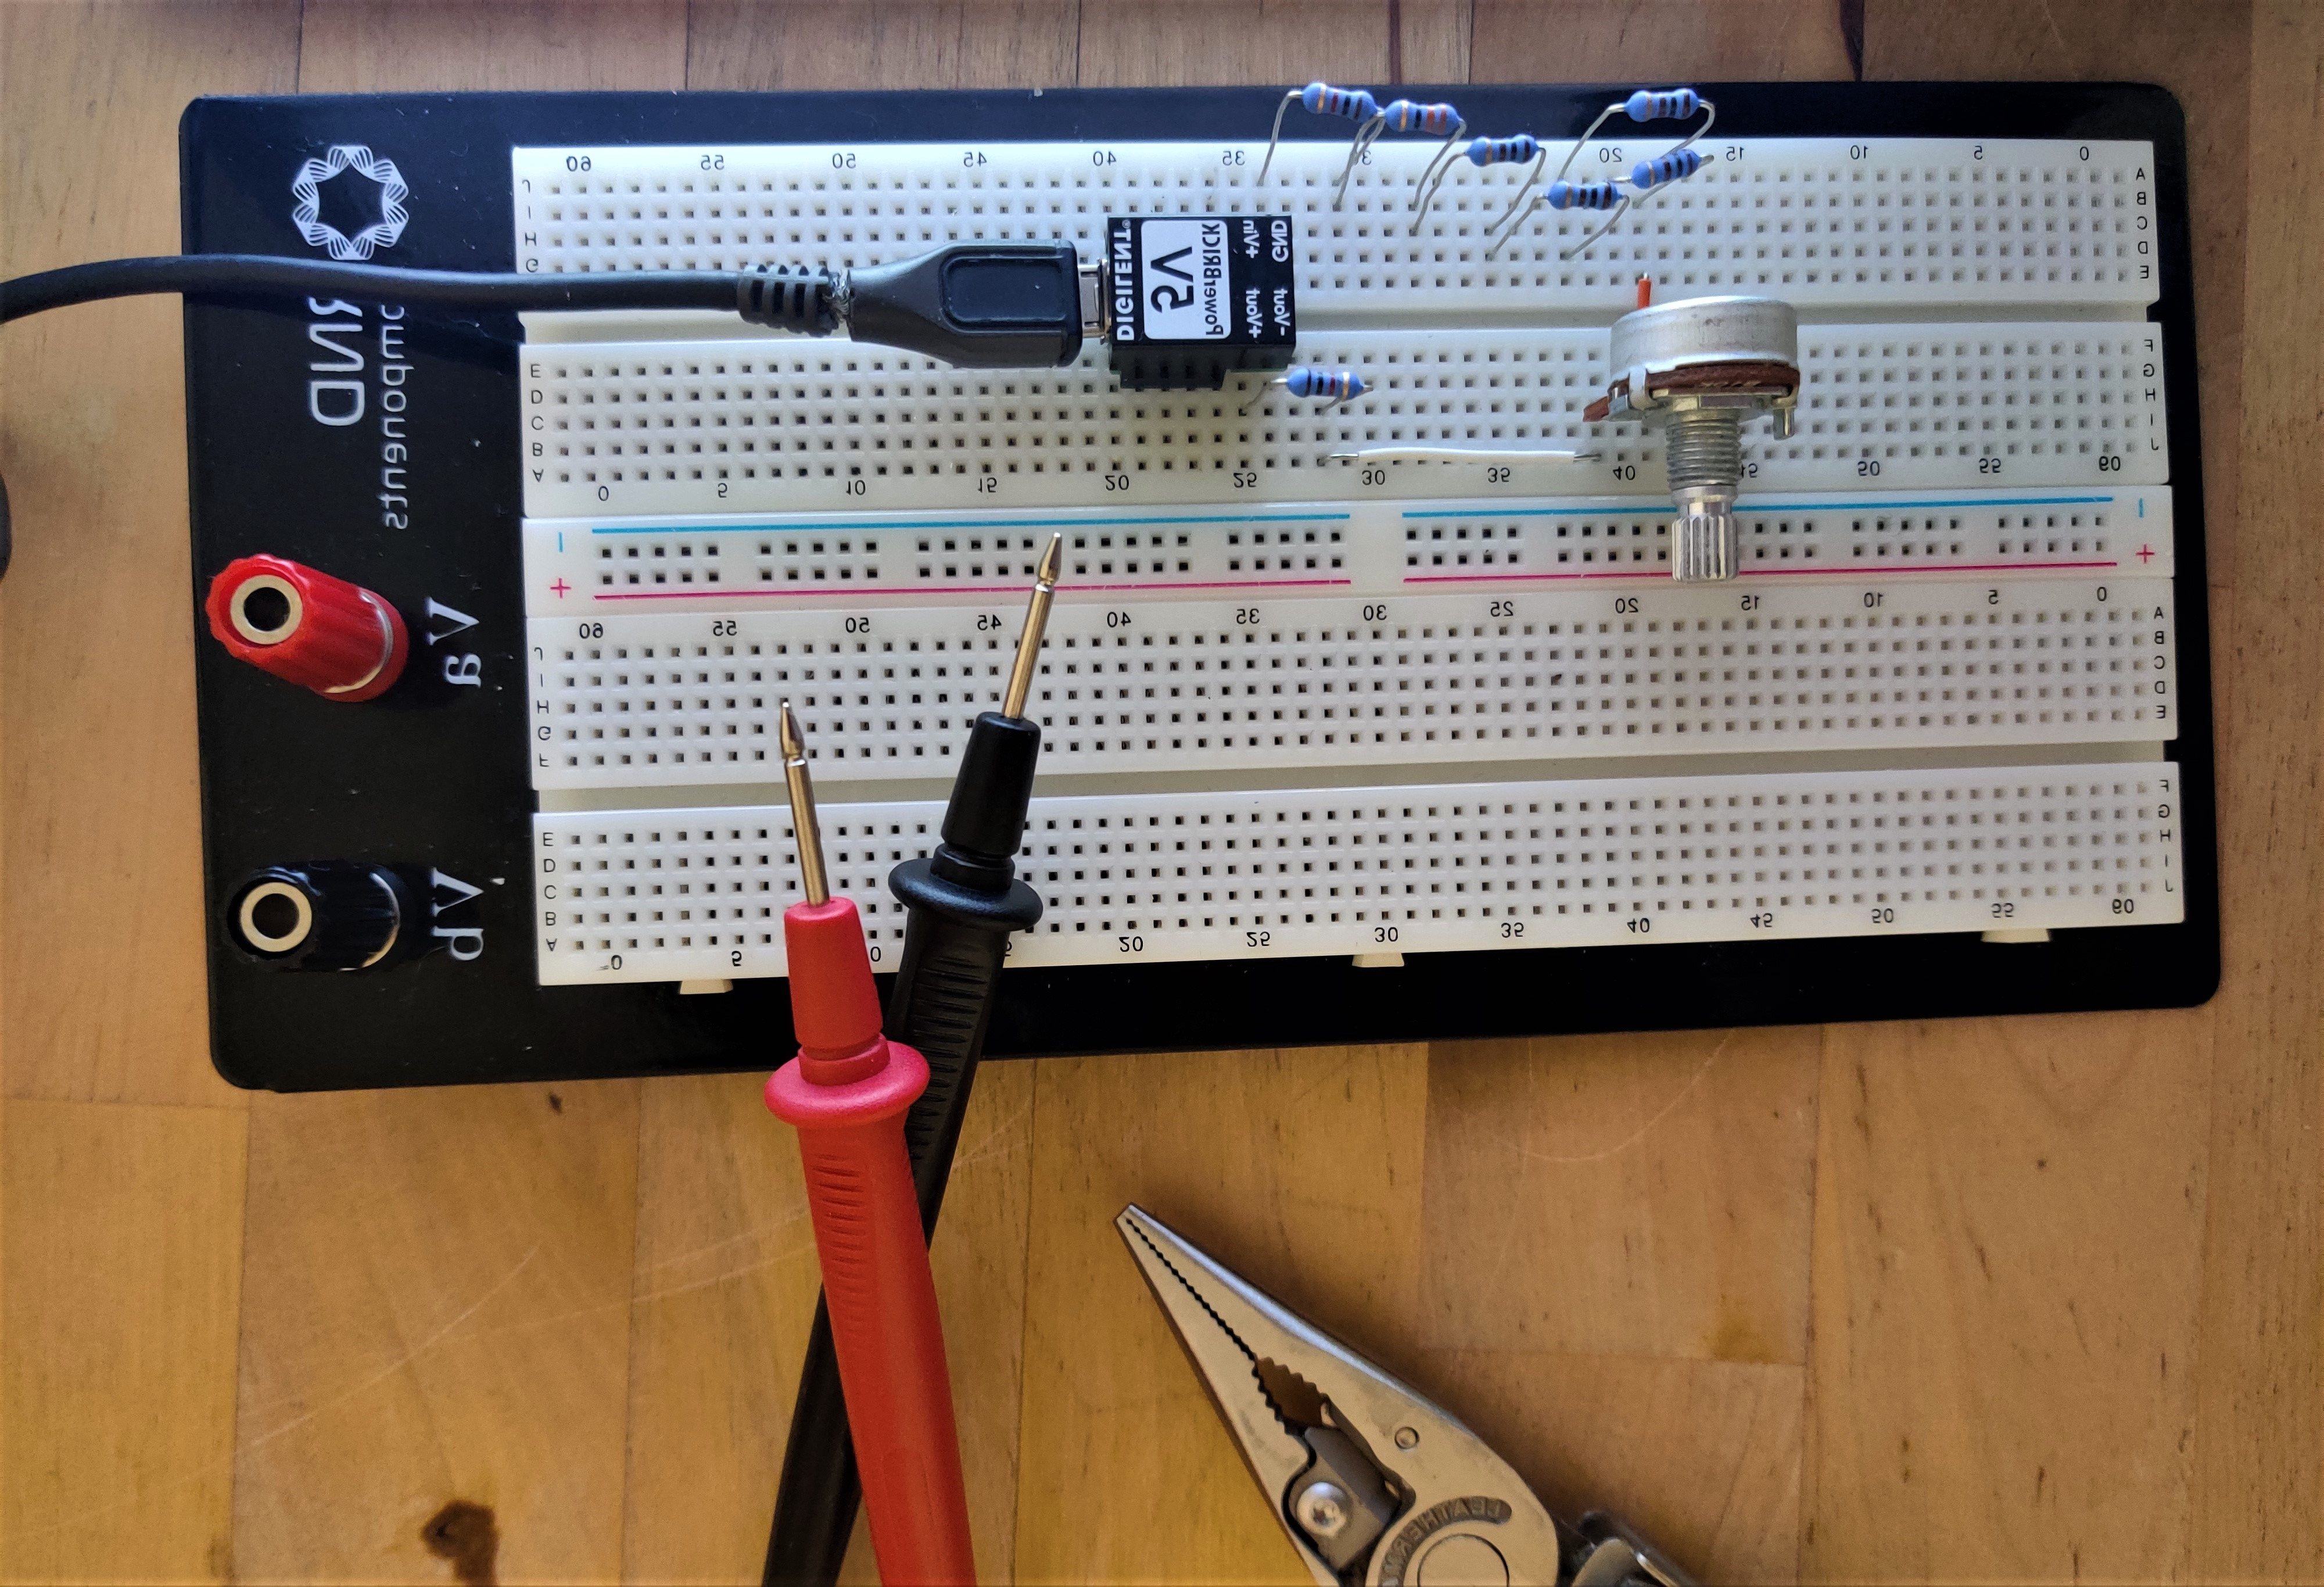
\includegraphics[scale=0.2]{D1/Images/oppkobling.jpg}
  \caption{Oppkobling av realisert krets på koblingsbrett.}
  \label{fig:oppkobling}
\end{figure}

\begin{figure}[H]
  \centering
  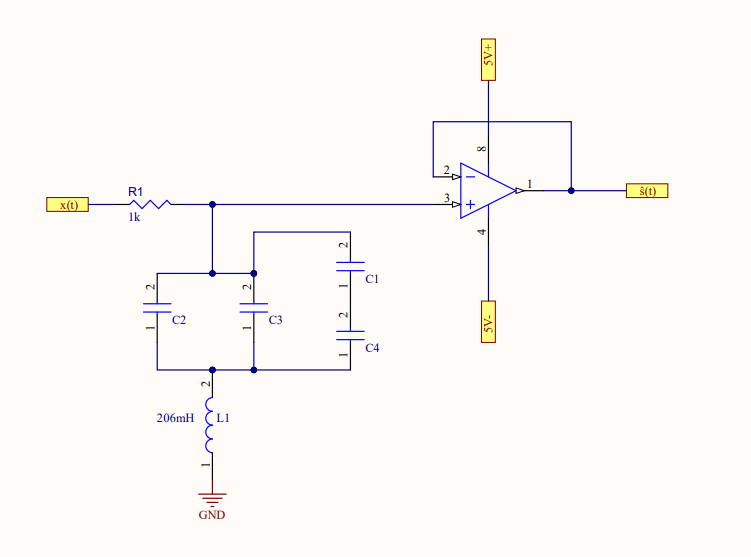
\includegraphics[scale=0.95]{D1/Images/Schematic.png}
  \caption{Skjematisk fremstilling av realisert krets.}
  \label{fig:schematic}
\end{figure}


\begin{table}[h]
  \centering
  \caption{Komponenter og deres standardverdier, samt målte verdier.}
  \label{tab:komp}
  \begin{tabular}{|c|c|c|}
    \hline\hline
    Komponenter & Standardverdi & Målt verdi \\
    \hline\hline
    $R_1$   & $0-10k\Omega$ & $8350\Omega$\\
    \hline
    $C_1$   & $100nF$       & $97nF$\\
    \hline
    $C_2$   & $100nF$       & $103nF$\\
    \hline
    $C_3$   & $100nF$       & $102nF$\\
    \hline
    $C_4$   & $100nF$       & $101nF$\\
    \hline
    $C_{sum}$   & $400nF$       & $403nF$\\
    \hline
    $L_1$   & $100mH$       & $206mH$\\
    \hline
    $LF353P$&&\\
    \hline\hline
  \end{tabular}
\end{table}
\subsection{Test}
Test av hvordan systemet fungerte ble gjennomført ved hjelp av en nettverksanalysator. Figur \ref{fig:netverk} viser frekvensresponsen til det realiserte systemet med amplitude- og faserespons plottet i et bodediagram. 

\begin{figure}[H]
  \centering
  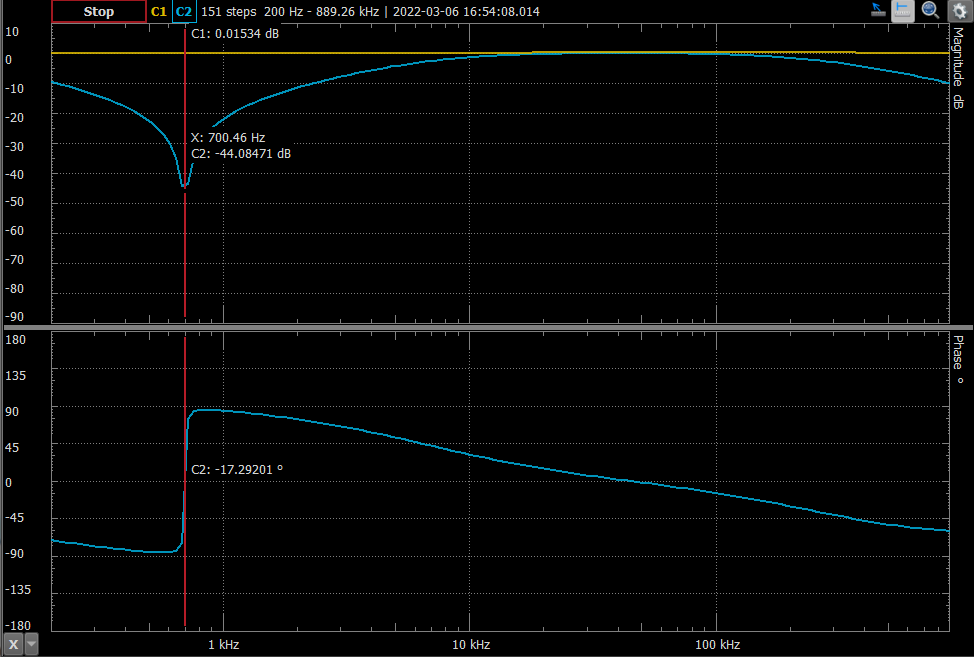
\includegraphics[scale=0.7]{D1/Images/network.png}
  \caption{Bodediagram som viser frekvensresponsen til realisert system, med amplitude- og faserespons.}
  \label{fig:netverk}
\end{figure}

Bodediagrammet viser at $f_C$ ved $700Hz$ er dempet med $-44dB$. Pipetonen er fremdeles tilstedet, men mye svakere. Frekvensene rundt $f_C$ er også betydelig dempet, noe som gir et svakere signal på $\hat{s}(t)$.


\section{Konklusjon}
\label{sec:konklusjon}

Systemet som ble beskrevet og implementert i dette notatet var et støyfjerningsfilter. Hensikten til dette systemet var å dempe en tidligere identifisert frekvens $f_C$ som lagde en pipetone i et lydsignal, men beholde resterende frekvenser mest mulig uendret. 
Etter testing og realisering ble $f_C$ dempet med $-44dB$, men frekvenser rundt $f_C$ ble også betydelig dempet. 

En løsning på dette kunne vært å bruke en lavere verdi for motstanden $R$ og heller lagt flere filter i serie. Det finnes også andre typer båndstopp-filter med smalere båndbredde, men disse blir fort mer avansert matematisk. 

\section{Takk}

Takk til Orbit NTNU for å gi meg muligheten til bruk av lokalet og alt nødvendig utstyr, samt hjelp av flere medlemmer. 

Takker også mine medstudenter Mahdan Gazimagamev og Nikolai Andresen for hjelp til feilsøking, oppkobling og produktiv diskusjon rundt prosjektet.

\phantomsection
\addcontentsline{toc}{section}{Referanser}

\begin{thebibliography}{99}
    \bibitem{notat}
        Lundheim L., 
        \textit{Teknisk notat: Enkle prinsipper for støyfjerning}, 
    	Elsys-2016-LL-2, 
    	NTNU,
    	2016.
    \end{thebibliography}
\end{document}